Action Geometry

the idea

shapes

\begin{figure}
	\centering
	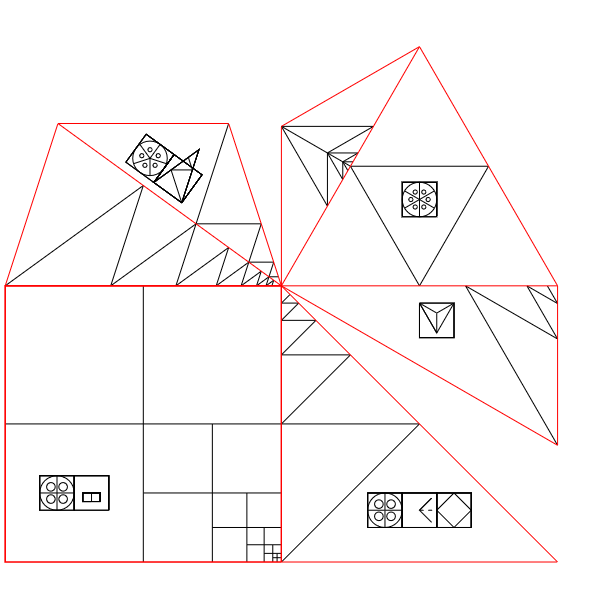
\includegraphics[width=3in]{figures/actiongeometry/shapeset.png}
	\caption[shapeset]
	{Shape Set. This is the basic shape set of Action Geometry.  It has the symmetries and scales of Geometron. What is shown should be printed exactly 6 inches wide, making each shape three inches on a side.}
\end{figure}

\begin{figure}
	\centering
	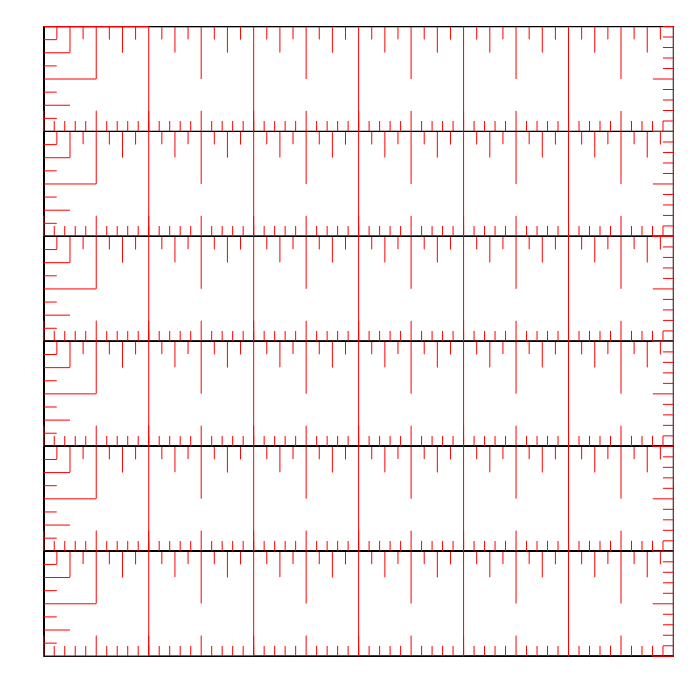
\includegraphics[width=3in]{figures/actiongeometry/rulers.png}
	\caption[rulers]
	{Rulers.  Make this 6 inches wide and each ruler is a 6 inch ruler, 1 inch across, with both tenth and factor of two divisions.}
\end{figure}

\begin{figure}
	\centering
	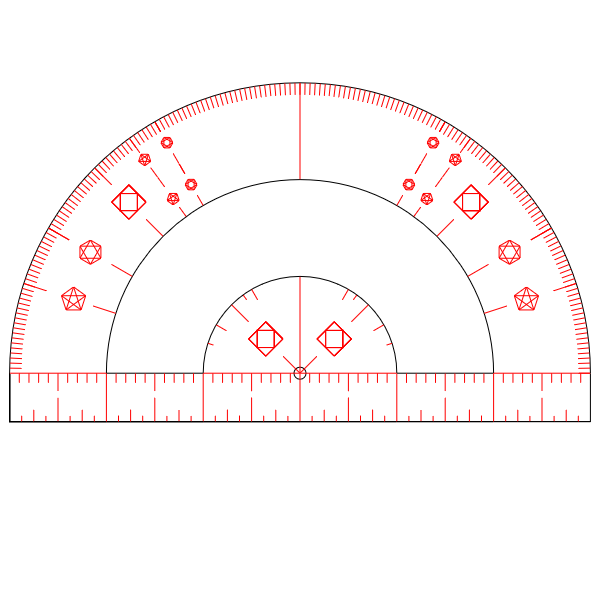
\includegraphics[width=3in]{figures/actiongeometry/protractor.png}
	\caption[protractor]
	{Geometron protractor.  While not really needed for Action Geometry, this protractor is a nice accessory which emphasizes Geometron symmetries rather than numbers, and allows drawing of circles of radius 3,2 and 1 inch without a compass.  This is mostly useful if cut out with a laser cutter.}
\end{figure}


\begin{figure}
	\centering
	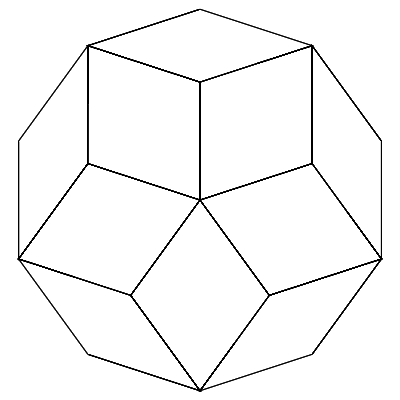
\includegraphics[width=3in]{figures/actiongeometry/penrose.png}
	\caption[penrose]
	{Penrose. Penrose tiles, the rhombi construction.}
\end{figure}

\begin{figure}
	\centering
	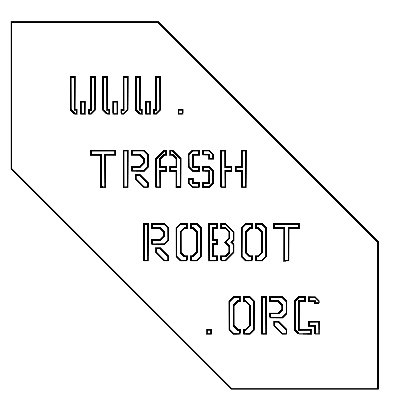
\includegraphics[width=3in]{figures/actiongeometry/stencil.png}
	\caption[stencil]
	{Spray paint stencil for laser cutting. You can use the Geometron software, selecting the built in laser font, to make a custom spray paint stencil pointing to the domain name which points to your Geometron server.  If you are Trash Robot, that can be Trash Robot, but we mostly point to a local non-property place.}
\end{figure}


\begin{figure}
	\centering
	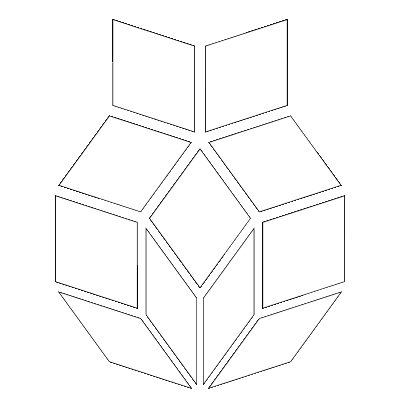
\includegraphics[width=3in]{figures/actiongeometry/pilogo.png}
	\caption[pilogo]
	{Construction of the Raspberry Pi logo for server bags. The top two shapes are green the rest are red.}
\end{figure}


products


\begin{figure}
	\centering
	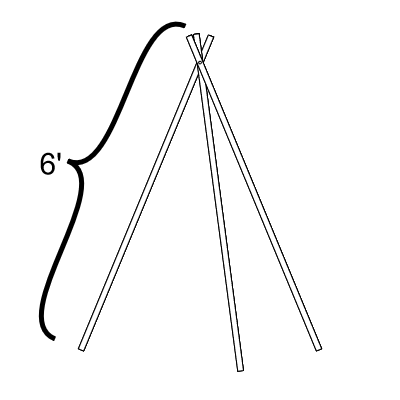
\includegraphics[width=3in]{figures/actiongeometry/skeletrontripod.png}
	\caption[skeletrontripod]
	{Skeletron tripod.  Three 6 foot bamboo trash poles wrapped in rainbow colored duct tape with quarter inch holes drilled just back from the end.  An 18 inch nylon parachute cord trash tie is used with a square knot to secure the top.  Many things can be hung from this, including servers, terminals, robots, boxes, flags, lights, textile arts and pendants on more trash ties.  The tripod can be carried over the shoulder to be mobile, without untying the joint at the top for rapid deployment.}
\end{figure}

\begin{figure}
	\centering
	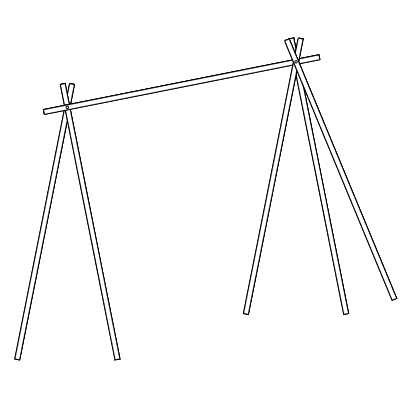
\includegraphics[width=3in]{figures/actiongeometry/skeletron2.png}
	\caption[skeletron2]
	{Skeletron cross bar configuration.  Two tripods can be converted into this stable configuration quickly to have a horizontal cross bar which S-Hooks can hang from to hang numerous objects of all kinds.}
\end{figure}


\begin{figure}
	\centering
	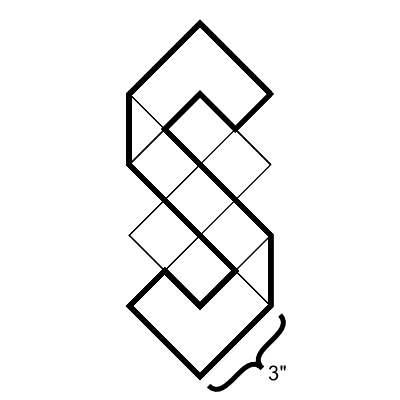
\includegraphics[width=3in]{figures/actiongeometry/shook.png}
	\caption[shook]
	{S-Hook.  Note the repeated use of the square shape, and the use of the 45 degree triangle, making this easy to replicate using the Shape Set.  This hook is used to hang things from the Trash Poles in Skeletron. Fabricate by stacking 4 identical layers of corrugated cardboard cut in this pattern and wrapping them in rainbow colored duct tape.  Googly eyes can then be applied.}
\end{figure}


\begin{figure}
	\centering
	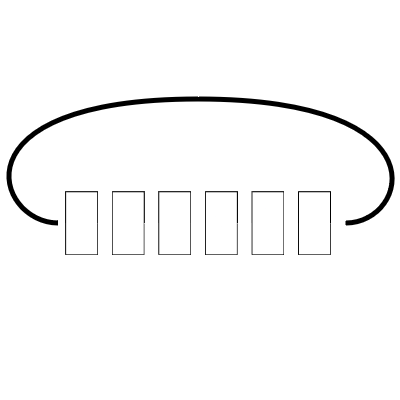
\includegraphics[width=3in]{figures/actiongeometry/tapesnake.png}
	\caption[tapesnake]
	{Tape Snake.  Duct tape rolls of all useful colors, namely the rainbow colors plus black and pink, are strung on a 6 foot Trash Tie made from a clothesline which is looped through twice and secured with a square knot in a bight(like a bow on a tied shoe) for rapid replacement of rolls as they are used.}
\end{figure}


\begin{figure}
	\centering
	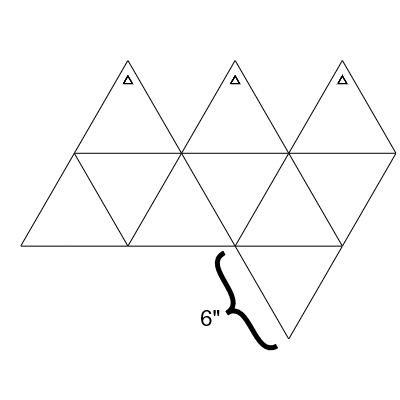
\includegraphics[width=3in]{figures/actiongeometry/artboxnet.png}
	\caption[artboxnet]
	{ArtBox Net.  Cut out 10 equilateral triangles from corrugated cardboard.  Duct tape the joints as shown.}
\end{figure}

\begin{figure}
	\centering
	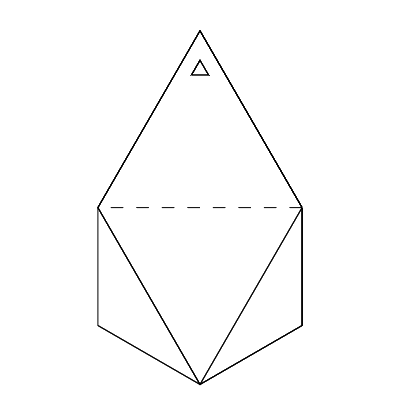
\includegraphics[width=3in]{figures/actiongeometry/artbox.png}
	\caption[artbox]
	{ArtBox assembly.  The fully assembled box is a tetrahedron on an octahedron.  It should contain the means of its own replication, which is a box cutter, a ruler, an equilateral triangle, and a sharpie, along with a Tape Snake for duct tape fabrication, extra Trash Ties, and googly eyes.  Use duct tape colors in sequence to create a fully rainbowed effect, then apply googly eyes and add a black duct tape mouth.}
\end{figure}

\begin{figure}
	\centering
	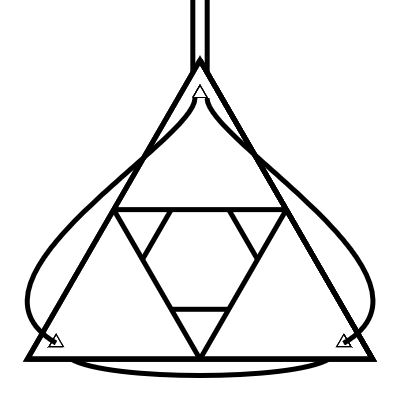
\includegraphics[width=3in]{figures/actiongeometry/artboxtop.png}
	\caption[artboxtop]
	{Top view of ArtBox.  Cut out little triangles in each of the top three petal triangles with the box cutter.  Thread a 6 foot Trash Tie with ends taped with duct tape as shown, and tie off the two bitter ends with a double figure eight knot for convenient purse-strap geometry.}
\end{figure}


\begin{figure}
	\centering
	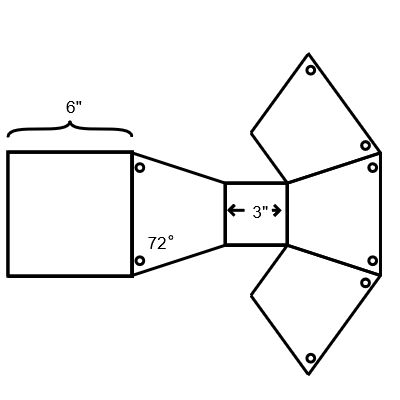
\includegraphics[width=3in]{figures/actiongeometry/pyramidnet.png}
	\caption[pyramidnet]
	{Pyramid net.  Use the Shape Set and Ruler to cut out corrugated cardboard patterns and stitch together with duct tape as shown.  Cutouts include a 6 inch square, a 3 inch square, and four trapezoids with 3 inch top and 6 inch base with 72 degree angles on the bottom angles.}
\end{figure}

\begin{figure}
	\centering
	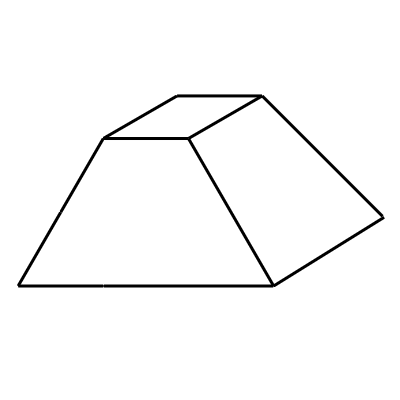
\includegraphics[width=3in]{figures/actiongeometry/pyramid.png}
	\caption[pyramid]
	{Pyramid assembly.  Fold it all up and then cover the whole thing in a skin of rainbow duct tape.  Open the base, insert technology and re-seal.  Add cutouts as needed for cords in and out.}
\end{figure}

the geometry, relation to geometron

shapes and rulers, protractors, laser cutting

methods of construction

materials

skeletron

artbox

pyramid

\begin{figure}
	\centering
	
\includegraphics[width=3in]{figures/shapes/blank.png}
    \caption[bags]
	{Bags are cut from black cloth, which can be scrap.  Black cloth bags are sewn up with Trash Ties as draw strings.}
\end{figure}


\begin{figure}
	\centering
	
\includegraphics[width=3in]{figures/shapes/blank.png}
    \caption[outfit]
	{Draw your personal Geometron outfit which is black with solid rainbow color felt or similar cloth sewn on in geometric patterns and geometric font.}
\end{figure}
\begin{figure}
	\centering
	
\includegraphics[width=3in]{figures/shapes/blank.png}
    \caption[outfit]
	{Draw your Flag.  A Flag is a black square cloth about 3 feet on a side, with a sewn hem with loops to tie a trash tie.  It is decorated with solid block letters and geometric shapes cut from solid color rainbow felt or similar.  All elements can be from scrap.  Flags point to domains in places.} 
\end{figure}
